%%%%%%%%%%%%%%%%%%%%%%% file template.tex %%%%%%%%%%%%%%%%%%%%%%%%%
%
% This is a general template file for the LaTeX package SVJour3
% for Springer journals.          Springer Heidelberg 2010/09/16
%
% Copy it to a new file with a new name and use it as the basis
% for your article. Delete % signs as needed.
%
% This template includes a few options for different layouts and
% content for various journals. Please consult a previous issue of
% your journal as needed.
%
%%%%%%%%%%%%%%%%%%%%%%%%%%%%%%%%%%%%%%%%%%%%%%%%%%%%%%%%%%%%%%%%%%%
%
% First comes an example EPS file -- just ignore it and
% proceed on the \documentclass line
% your LaTeX will extract the file if required
\begin{filecontents*}{example.eps}
%!PS-Adobe-3.0 EPSF-3.0
%%BoundingBox: 19 19 221 221
%%CreationDate: Mon Sep 29 1997
%%Creator: programmed by hand (JK)
%%EndComments
gsave
newpath
  20 20 moveto
  20 220 lineto
  220 220 lineto
  220 20 lineto
closepath
2 setlinewidth
gsave
  .4 setgray fill
grestore
stroke
grestore
\end{filecontents*}
%
\RequirePackage{fix-cm}
%
\documentclass[twocolumn]{svjour3}         % twocolumn
%\documentclass[smallcondensed]{svjour3}     % onecolumn (ditto)
%\documentclass[smallextended]{svjour3}       % onecolumn (second format)
%\documentclass{svjour3}                     % onecolumn (standard format)
%
\smartqed  % flush right qed marks, e.g. at end of proof
%
%
% \usepackage{mathptmx}      % use Times fonts if available on your TeX system
%
% insert here the call for the packages your document requires
\usepackage{graphicx}
\graphicspath{{../}{./}}
\usepackage{booktabs}
\usepackage{amsmath,amssymb}
\usepackage{algorithm}
\usepackage{algpseudocode}
\usepackage[hidelinks]{hyperref}
\usepackage{array}
\usepackage{enumitem}
\usepackage{microtype}
\usepackage{xspace}
\usepackage{CJKutf8}
\setlength{\textfloatsep}{10pt plus 2pt minus 2pt}
\setlength{\floatsep}{8pt plus 2pt minus 2pt}
\setlength{\intextsep}{8pt plus 2pt minus 2pt}
\emergencystretch=1.5em

\newcommand{\algname}{ReRAPTOR\xspace}
\newcommand{\ind}{\mathbb{I}}
%\usepackage{latexsym}
% etc.
%
% please place your own definitions here and don't use \def but
% \newcommand{}{}
%
% Insert the name of "your journal" with
\journalname{ITS Symposium}
%
\begin{document}

\title{ReRAPTOR: Reverse-Objective RAPTOR for Time-Budgeted Value-Maximizing Transit Itinerary Planning}
%\subtitle{Subtitle}

\titlerunning{ReRAPTOR for Value-Maximizing Transit Itinerary Planning}

\author{Bin Zhou \and
    Guangxian Li \and
    Teruki Ogo \and
    Yutaka Arakawa \and
    Tsunenori Mine %etc.
}

%\authorrunning{Short form of author list} % if too long for running head

\institute{Bin Zhou and Guangxian Li \at
    Graduate School of Information Science and Electrical Engineering, Kyushu University, Fukuoka, Japan \\
    \email{zhou.bin.883@s.kyushu-u.ac.jp; li.guangxian.021@s.kyushu-u.ac.jp}
    \and
    Teruki Ogo \at
    Faculty of Information Science and Engineering, Kyushu Sangyo University, Fukuoka, Japan \\
    \email{k25rm021@st.kyusan-u.ac.jp}
    \and
    Yutaka Arakawa and Tsunenori Mine \at
    Faculty of Information Science and Electrical Engineering, Kyushu University, Fukuoka, Japan \\
    \email{arakawa@ait.kyushu-u.ac.jp; mine@ait.kyushu-u.ac.jp}
}

\date{Received: date / Accepted: date}
% The correct dates will be entered by the editor


\maketitle

\begin{abstract}
    Conventional public-transit routing prioritizes arrival time, whereas a
    leisure itinerary may instead need to maximize collected value under a hard
    time budget. We formulate this timetable-constrained problem and propose
    ReRAPTOR, a heuristic search in the Round-bAsed Public Transit Optimized
    Router (RAPTOR) family that preserves schedule
    feasibility while ranking partial itineraries by a pluggable value model.
    Candidate trimming and bucket beam jointly form a two-stage Beam layer;
    heuristic Dominance removes locally weaker labels, and an optional penalty
    down-ranks undesirable route patterns. On Fukuoka timetable data, a seeded
    stop-reward benchmark
    compares ReRAPTOR with nine routing and metaheuristic baselines. ReRAPTOR has
    the highest mean Stop Score (\(872.438\)), \(8.710\%\) above the
    non-dominated sorting genetic algorithm II (NSGA-II), while
    NSGA-II requires \(6.89\times\) as much generation time on average. This
    aggregate gain is associated mainly
    with reaching more distinct scored stops and returning feasible routes more
    reliably; among tasks on which every NSGA-II run succeeds, the score
    difference is inconclusive. Ablation identifies the Beam layer and Dominance as the
    main scalability controls. Sensitivity results are unchanged for
    \(W\geq25\) and all tested label-ranking coefficients, whereas the candidate
    cap governs the quality--resource trade-off. These results establish a
    strong overall balance on the tested network, not universal superiority.
    \keywords{Transit itinerary planning \and Transit schedule data \and RAPTOR \and Time-budgeted route planning \and Multi-objective search}
    % \PACS{PACS code1 \and PACS code2 \and more}
    % \subclass{MSC code1 \and MSC code2 \and more}
\end{abstract}

\section{Introduction}
Public-transit routing usually seeks earliest-arrival or Pareto-efficient
journeys \cite{agarwal2024bicriteriontb,delling2019restrictedpareto,delling2015raptor,he2022paretojourneys}.
For leisure travel, however, a user may want the most rewarding itinerary that
can be completed within a fixed time. Its value may depend on the stops already
visited, their rewards, and the order in which they are reached. This task is
therefore closer to budgeted itinerary design than to shortest-path search
\cite{gunawan2016survey,ruizmeza2022slr,souffriau2008personalized}.

Combining a timetable with a history-dependent objective creates a specific
search problem. Every extension must respect scheduled departures, arrivals,
and transfers, yet partial itineraries that reach the same stop can have
different collected value and future opportunities. Keeping only the earliest
arrival can discard a valuable history; keeping every history causes rapid
label growth. Existing timetable routers and value-maximizing trip planners
address the two sides of this problem, but their usual state and search controls
do not directly resolve this tension.

We address the gap with ReRAPTOR, a reverse-objective RAPTOR-style search over
timetable schedules \cite{delling2015raptor,wessel2017retrospective,wong2013leveraginggtfs}.
Here \emph{reverse-objective} does not mean reversing time or graph direction.
It means retaining timetable feasibility as a hard constraint while making
route value, rather than earliest arrival, the primary ranking objective.
ReRAPTOR carries the history required by a pluggable value module and controls
the resulting state growth through a two-stage Beam layer (candidate trimming
and bucket beam), heuristic Dominance, and optional penalty-based down-ranking.

We ask whether ReRAPTOR improves the quality--time balance and where it loses,
which controls produce its behavior, and whether fixed hyperparameters drive
the conclusion. A reproducible Fukuoka benchmark with nine baselines, a full
ablation, 22 sensitivity configurations, and three route cases answers these
questions. The contributions are a formal value-maximizing timetable problem,
an explicit pluggable search algorithm, and evidence that separates aggregate
performance, mechanism, robustness, and limits. ReRAPTOR is heuristic: it
searches a controlled subset of feasible itineraries and has no global
optimality guarantee.

\section{Related Work}
Round-Based Public Transit Optimized Router (RAPTOR) is a round-based framework
for earliest-arrival and multicriteria transit
routing \cite{delling2015raptor}. Later work improves transfers, restricted
Pareto search, and acceleration
\cite{abuaisha2024transferdb,agarwal2024bicriteriontb,delling2019restrictedpareto,delling2017hyperpartitioning,he2022paretojourneys,phan2019hublabeling}.
Fare-aware and broader multi-objective variants have also been studied
\cite{euler2024price,weng2021mcts}, supported by the General Transit Feed
Specification (GTFS) and related timetable
datasets \cite{godfrid2022mobilitydb,kujala2018datasets,pereira2022gtfs2gps,wong2013leveraginggtfs}.
These methods make timetable routing efficient, but do not directly optimize
history-dependent route value under a fixed total budget.

Tourist trip design and orienteering instead maximize collected value under
time constraints \cite{gavalas2015teamorienteering,gunawan2016survey,ruizmeza2022slr,souffriau2008personalized}.
Preference-aware route systems extend this idea to personalized and multimodal
settings \cite{persia2020socialsensing,pilato2023modular,zhang2025dynamicmultimodal,xia2024integrated}.
General optimizers such as the nondominated sorting genetic algorithm II
(NSGA-II), iterated local search (ILS), variable
neighborhood search (VNS), and simulated annealing (SA) are also relevant
\cite{deb2002nsga2,kirkpatrick1983sa,lourenco2003ils,mladenovic1997vns}.
ReRAPTOR differs by optimizing value during timetable-feasible expansion, not
only after full itineraries have been constructed.

\section{Problem Formulation}
Let \(G=(\mathcal{S},\mathcal{E})\) be a timetable graph, where \(\mathcal S\)
is the stop set and \(\mathcal E\) is the set of scheduled ride edges. An edge
\(e=(u,v,\tau^{\rm dep},\tau^{\rm arr},p,\ell)\) has origin \(u(e)=u\),
destination \(v(e)=v\), departure and arrival times, trip \(p\), and line
\(\ell\). A query \(q=(o,t_0,B)\) gives the origin, earliest departure, and time
budget. A route \(r=(e_1,\ldots,e_m)\), where \(m\geq1\) is its number of
scheduled ride legs, is timetable-feasible when the two inter-leg conditions
below hold for \(i=1,\ldots,m-1\):
\begin{equation}
    \label{eq:feasibility}
    \begin{aligned}
        u(e_1)&=o,\qquad \tau^{\rm dep}(e_1)\ge t_0,\\
        v(e_i)&=u(e_{i+1}),\\
        \tau^{\rm dep}(e_{i+1})&\ge\tau^{\rm arr}(e_i)+\delta(e_i,e_{i+1}),\\
        \tau^{\rm arr}(e_m)\le t_0+B .
    \end{aligned}
\end{equation}
Here \(\delta(e_i,e_{i+1})=0\) if both rides remain on the same trip and line,
and equals the minimum transfer time \(\Delta_{\rm tr}\) otherwise. An objective module
identified by \(\theta\) supplies a complete-route value \(F_\theta(r)\), a
resource function
\(T_\theta\) for partial and complete routes, a partial-label ranking score
\(S_\theta\), objective-state updates, and a Boolean acceptance rule
\(A_\theta(r)\). Let \(\mathcal R_\theta(q)\) contain the routes that satisfy
Eq.~\ref{eq:feasibility}, \(T_\theta(r)\leq B\), and \(A_\theta(r)=1\). The
target problem is
\begin{equation}
    \label{eq:target_problem}
    r^*\in\arg\max_{r\in\mathcal R_\theta(q)}F_\theta(r).
\end{equation}
This interface separates the task definition from the common timetable search.

Experiments~1--3 use a seeded stop-reward module. Each stop receives a fixed
reward \(w_\omega(s)\). Let \(V(r)\) be the set of stops in \(r\),
\(V^+(r)=V(r)\setminus\{o\}\), and
route elapsed time \(T(r)=\tau^{\rm arr}(e_m)-t_0\), which includes initial
waiting.
Every unique non-origin stop also incurs a per-stop effective-time charge
\(\eta\). This is a resource-accounting charge, not physical dwell inserted
into the timetable. The effective time and complete-route value are
\begin{equation}
    \label{eq:objective_stop_reward}
    \begin{aligned}
        T_\eta(r)&=T(r)+\eta|V^+(r)|,\qquad T_\eta(r)\le B,\\
        F_{\omega,\eta}(r)&=\sum_{s\in V^+(r)}w_\omega(s).
    \end{aligned}
\end{equation}
The seed \(\omega\) fixes one reward map. Replacing the reward with an attraction
rating or other utility changes the module, not timetable feasibility.
\(A_{\omega,\eta}\) accepts a resource-feasible route with at least two legs.
The per-stop charge is added only to the resource budget and does not shift the
scheduled connection times in Eq.~\ref{eq:feasibility}.

\section{Proposed Method}
\subsection{Labels and Timetable-Feasible Expansion}
ReRAPTOR uses RAPTOR-style round buckets but expands scheduled ride segments
directly \cite{delling2015raptor,he2022paretojourneys}. Here a \emph{round} is
one leg-extension depth, not the transfer-count round of the original RAPTOR
algorithm. A label
\begin{equation}
    \label{eq:label}
    \lambda=(v,a,k,\pi,\mathbf c,\rho,z_\theta,s_\theta)
\end{equation}
stores current stop \(v\), arrival time \(a\), leg count \(k\), a predecessor
chain \(\pi\), stop-visit counts \(\mathbf c\), accumulated in-vehicle minutes
\(\rho\), objective state \(z_\theta\), and its cached ranking score
\(s_\theta=S_\theta(\lambda)\). The predecessor
chain determines the ordered route \(r(\lambda)\) and its last trip. For the stop-reward
module, \(z_{\omega,\eta}=(V^+,\sigma)\), where
\(\sigma=\sum_{s\in V^+}w_\omega(s)\). Bucket \(\mathcal L_k(v)\) contains
labels at stop \(v\) after \(k\) legs; \(\mathcal M_k\) is the set of stops
whose round-\(k\) buckets still require expansion.

The initial label \(\lambda_0\) has \(v=o\), \(a=t_0\), \(k=0\),
\(\pi=\varnothing\), \(\rho=0\), the module's zero objective state, and
\(s_\theta=S_\theta(\lambda_0)\). For the stop-reward module,
\(V^+=\varnothing\), \(\sigma=0\), \(c_o=1\), and \(c_s=0\) for every
\(s\in\mathcal S\setminus\{o\}\).

An extension appends a scheduled edge only when its origin is \(v\), its
departure satisfies Eq.~\ref{eq:feasibility}, and the updated
objective-specific resource remains feasible. In the stop-reward module, the
partial effective time is \(T_\eta(\lambda)=a-t_0+\eta|V^+|\). A first visit
adds its reward and the per-stop effective-time charge; a repeated visit adds
neither. This state retains
information that an earliest-arrival label alone cannot represent.

\begin{figure*}[t]
    \centering
    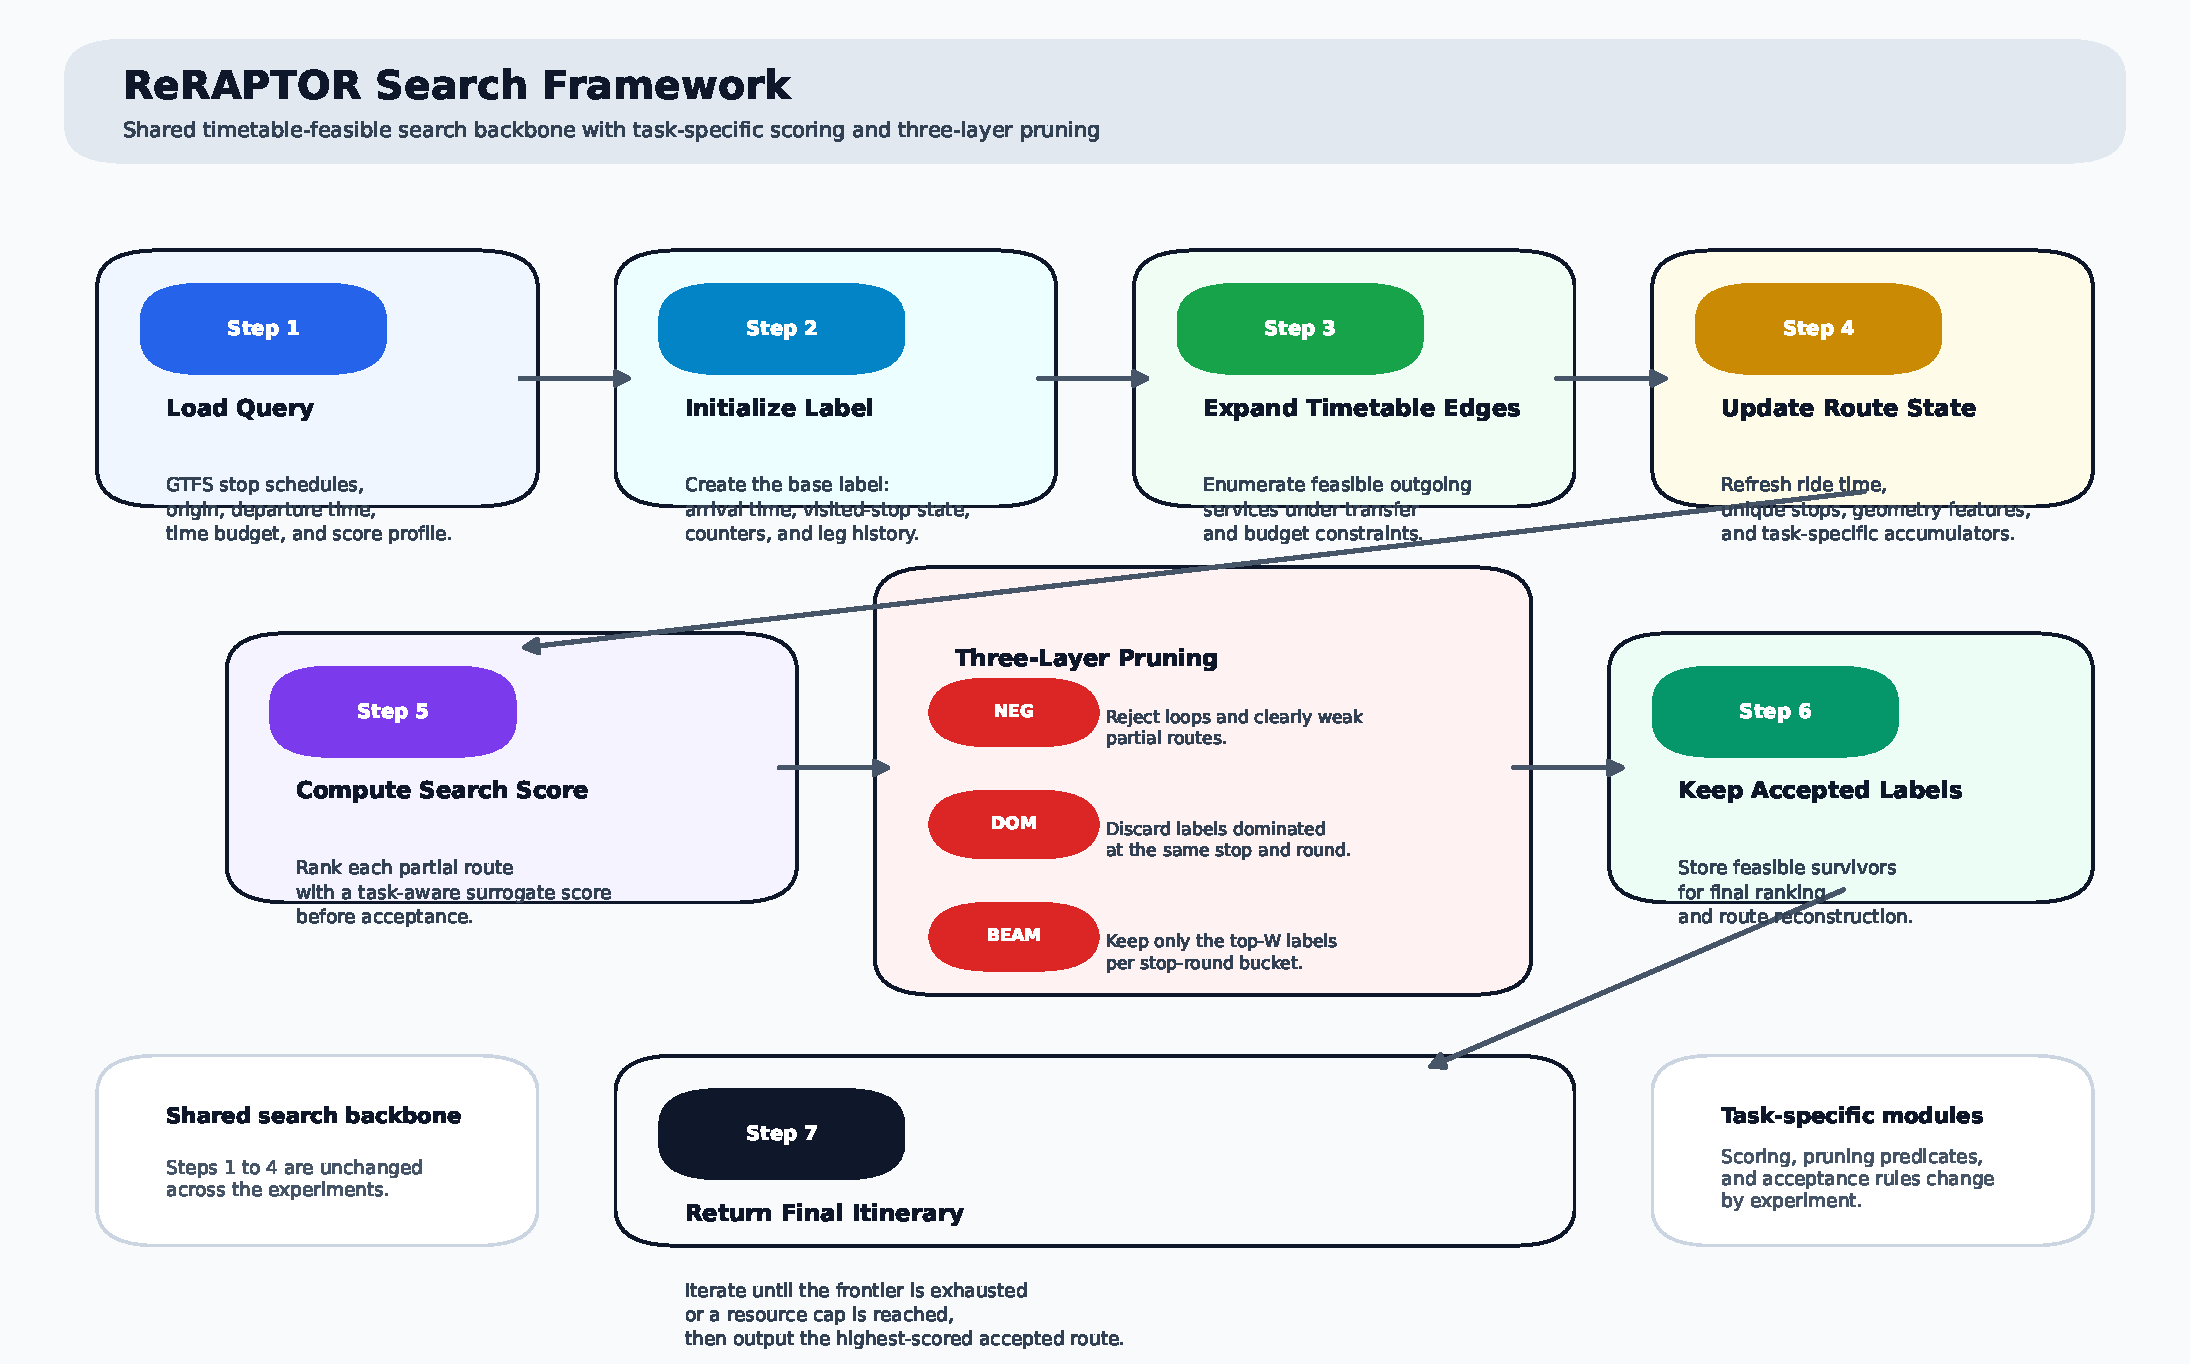
\includegraphics[width=0.94\textwidth]{figures/method/ours_framework_flow.pdf}
    \caption{ReRAPTOR workflow. A common timetable-feasible search backbone uses
    a task-specific scoring and acceptance module; Experiment~2 disables the
    Beam layer, Dominance, and Negative down-ranking individually and in
    combination.}
    \label{fig:method_framework}
\end{figure*}

\subsection{Value Ranking and Search Control}
The objective module ranks every feasible partial label by
\begin{equation}
    \label{eq:search_score}
    S_\theta(\lambda)=\Phi_\theta(\lambda)-P(\lambda),
\end{equation}
where \(\Phi_\theta\) is the objective-specific surrogate before optional
route-pattern penalties. The term \(P\) only lowers rank; it does not make a
label infeasible. For the stop-reward task,
\begin{equation}
    \label{eq:search_score_stop_reward}
    \begin{aligned}
        S_{\omega,\eta}(\lambda)={}&10000\sigma+5\,{\rm SPH}
        -0.1T_\eta(\lambda)\\
        &-50000[T_\eta(\lambda)-B]_+-P(\lambda),
    \end{aligned}
\end{equation}
where \([x]_+=\max(0,x)\). Score per hour
\({\rm SPH}=60\sigma/T_\eta(\lambda)\) when \(T_\eta(\lambda)>0\), and is zero
for the initial label. The hard feasibility check normally makes the budget
term zero; it remains a safeguard in the shared scorer. The route-pattern
penalty is
\begin{equation}
    \label{eq:negative_penalty}
    \begin{aligned}
    P(\lambda)={}&50000\ind\!\left[\max_{s\in\mathcal S} c_s>2\right]\\
    &+20000\ind\!\left[|V^+|>0\ \land\ \rho<2|V^+|\right],
    \end{aligned}
\end{equation}
where \(c_s\) is the visit count of stop \(s\), and \(\ind[\cdot]\) is one
when its condition holds and zero otherwise. The second condition is written
without division so that it is defined for the initial label, where
\(|V^+|=0\). We call this optional term \emph{Negative down-ranking}.
The reward term sets the main ordering, while SPH and effective time resolve
near-ties. These fixed coefficients are tested in Experiment~3.

The Beam layer limits growth in two stages. Candidate trimming gives same-trip
continuation first priority, then orders edges by the following objective score
and earlier schedule times. For edge \(e\), let
\(d_e=\tau^{\rm arr}(e)-\tau^{\rm dep}(e)+\eta\), let \(w_e=0\) when
\(v(e)=o\) and \(w_\omega(v(e))\) otherwise, and let \(\alpha_e=0.15\) when
\(v(e)\) has already been visited and 1 otherwise:
\begin{equation}
    \label{eq:edge_priority}
    \begin{aligned}
    H(e\mid\lambda)={}&\alpha_e w_e+
    25\frac{w_e}{\max(1,d_e)}-0.05\max(1,d_e)\\
    &+2\ind[\text{same trip}].
    \end{aligned}
\end{equation}
It keeps \(C(B)=30\) candidates for \(B\leq240\) min and 20 otherwise.
\emph{Heuristic Dominance} then compares labels in the same
stop--round bucket. Write \(\sigma(\lambda)\) for the accumulated reward stored
in the objective state of \(\lambda\). Then
\begin{equation}
    \label{eq:dominance_stop_reward}
    \begin{aligned}
    \lambda^a\succeq\lambda^b \iff{}&
    \sigma(\lambda^a)\geq\sigma(\lambda^b)
    \ \land\ T_\eta(\lambda^a)\leq T_\eta(\lambda^b)\\
    &\land\bigl(\sigma(\lambda^a)>\sigma(\lambda^b)
    \ \lor\ T_\eta(\lambda^a)<T_\eta(\lambda^b)\\
    &\hspace{20mm}\lor\ S_{\omega,\eta}(\lambda^a)>
    S_{\omega,\eta}(\lambda^b)\bigr).
    \end{aligned}
\end{equation}
Thus, an exact reward--time tie is resolved only by a strictly higher
\(S_{\omega,\eta}\). This rule is not Pareto-safe: it may discard a partial
label that could lead to a Pareto-optimal completed route because visited sets
and continuation states can differ. It is a deliberate heuristic reduction
\cite{demeyer2013martins,he2022paretojourneys}. The Beam layer's second stage,
bucket beam, keeps the best \(W=50\) labels by \(S_\theta\). Thus,
\texttt{NoBeam} disables both candidate trimming and bucket beam. The default
width is a preselected middle setting, not a fitted optimum.

In Algorithm~\ref{alg:reraptor}, \(v(e)\) is the edge destination;
\textsc{FeasibleEdges} applies timetable, lookahead, and budget tests;
\textsc{TopCandidates} applies \(H\) and \(C(B)\); \textsc{Extend} updates
Eq.~\ref{eq:label}; and \textsc{InsertND} applies Dominance, or always inserts
when it is disabled. \textsc{TopW} truncates its bucket in place to the \(W\)
largest-\(S_\theta\) labels. \textsc{Eligible} is true exactly when
\(A_\theta(r(\lambda))=1\) and
\([\lambda^{\rm best}=\varnothing\ \lor\
S_\theta(\lambda)>S_\theta(\lambda^{\rm best})]\).
The largest-\(S_\theta\) accepted label admitted by \textsc{InsertND} approximates
Eq.~\ref{eq:target_problem}; bucket trimming prevents later expansion of removed
labels but does not erase an accepted solution already observed.

\begin{algorithm}[t]
\caption{ReRAPTOR controlled value search}
\label{alg:reraptor}
\footnotesize
\begin{algorithmic}[1]
\Require \(q,\theta,W,C(B)\), and maximum depth \(R\)
\State initialize \(\mathcal L_0(o)=\{\lambda_0\}\), \(\mathcal M_0=\{o\}\), and \(\lambda^{\rm best}=\varnothing\)
\For{\(k=0,\ldots,R-1\)}
    \State \(\mathcal M_{k+1}\gets\varnothing\)
    \ForAll{\(v\in\mathcal M_k\) and \(\lambda\in\mathcal L_k(v)\)}
        \State \(E\gets\Call{FeasibleEdges}{\lambda,q}\)
        \If{candidate trimming is enabled} \State \(E\gets\Call{TopCandidates}{E,C(B),H}\) \EndIf
        \ForAll{\(e\in E\)}
            \State \(\lambda'\gets\Call{Extend}{\lambda,e,\theta}\)
            \If{\(T_\theta(\lambda')\le B\)}
                \State compute \(S_\theta(\lambda')\)
                \If{\Call{InsertND}{$\lambda',\mathcal L_{k+1}(v(e))$}}
                    \If{bucket beam is enabled}
                        \State \Call{TopW}{$\mathcal L_{k+1}(v(e)),W,S_\theta$}
                    \EndIf
                    \State \(\mathcal M_{k+1}\gets\mathcal M_{k+1}\cup\{v(e)\}\)
                    \If{\Call{Eligible}{$\lambda',\lambda^{\rm best},\theta$}}
                        \State \(\lambda^{\rm best}\gets\lambda'\)
                    \EndIf
                \EndIf
            \EndIf
        \EndFor
    \EndFor
    \If{\(\mathcal M_{k+1}=\varnothing\)} \State \textbf{break} \EndIf
\EndFor
\State \Return \(\lambda^{\rm best}\), or failure if none was accepted
\end{algorithmic}
\end{algorithm}

\subsection{Complexity and Implementation}
With both Beam stages enabled, let \(C_k(v,\lambda)\leq C(B)\) be the number of
candidate edges retained for label \(\lambda\in\mathcal L_k(v)\). The number
of attempted extensions is bounded by
\begin{equation}
    \label{eq:expansion_bound}
    N_{\rm ext}\leq\sum_{k=0}^{R-1}\sum_{v\in\mathcal M_k}
    \sum_{\lambda\in\mathcal L_k(v)}C_k(v,\lambda)
    \leq R|\mathcal S|WC(B).
\end{equation}
Dominance checks at most \(W\) labels per insertion, giving a conservative
\(O(R|\mathcal S|C(B)W^2)\) bound, excluding timetable lookup and objective
updates. Active buckets contain \(O(|\mathcal S|W)\) labels; retaining all
rounds gives \(O(R|\mathcal S|W)\) label records.

The reference implementation indexes outgoing schedules, uses a 120-min
schedule-query lookahead window (distinct from the Greedy baseline's \(L\)),
sets \(\Delta_{\rm tr}=3\) min, and limits depth to
\(R=\min(220,\max(40,\lfloor B/2\rfloor+20))\). Resource guards terminate a
run with its current best accepted label; their incidence is reported rather
than hidden.

\section{Experimental Evaluation}
\subsection{Common Data, Measures, and Protocol}
The experiments follow the questions stated in the Introduction. Experiment~1
evaluates quality, runtime, reliability, and conditions of underperformance;
Experiment~2 isolates the search controls; Experiment~3 tests
hyperparameters; and Experiment~4 explains representative route outcomes.

\paragraph{Baselines.}
Baseline selection follows three criteria: (1)~task compatibility with
timetable-feasible fixed-budget routing, (2)~reproducible implementation
in our evaluation pipeline, and (3)~diversity across optimizer families.
We therefore compare general-purpose metaheuristics (NSGA-II~\cite{deb2002nsga2},
ILS~\cite{lourenco2003ils}, VNS~\cite{mladenovic1997vns}, and
SA~\cite{kirkpatrick1983sa}), transit-routing baselines (multicriteria RAPTOR
(McRAPTOR), Pure RAPTOR~\cite{delling2015raptor}, and Greedy), and two recent
adapted methods described below. ILS uses a timetable-feasible 2-opt-like
cut-and-tail-regrowth neighborhood. Pure RAPTOR is the same scheduled-edge
expansion with Beam, Dominance, and Negative down-ranking disabled but a 60-s
guard retained. Greedy uses \(L=3\), the number of one-step onward candidates
included in its discounted lookahead.
Supplementary Table~S7 lists the fixed implementation parameters for all nine
baselines; the source files named there are the executable specifications.

\textbf{Adapted baselines.}
Adaptive large-neighborhood search (ALNS) and dynamic preference (DynPref)
address related systems. Table~\ref{tab:adapted_baselines} states what was
retained and changed. All methods use the same timetable, query grid and
execution order, reward maps, effective-time and transfer rules, route validator, and
zero-score failure policy. Methods that modify complete routes also use the
same timetable-feasible repair interface. Because iteration, stagnation, and
resource guards remain method-specific, search effort is not exactly equalized;
ALNS and DynPref are adaptations, not original-setting replications.

\begin{table*}[t]
    \centering
    \caption{Implementation of the two adapted baselines
    (\(u=T_\eta/B\): fraction of the effective-time budget used). Complete
    parameter files accompany the code.}
    \label{tab:adapted_baselines}
    \begingroup
    \scriptsize
    \setlength{\tabcolsep}{3pt}
    \renewcommand{\arraystretch}{1.05}
    \begin{tabular}{@{}>{\raggedright\arraybackslash}p{0.10\textwidth}
                    >{\raggedright\arraybackslash}p{0.24\textwidth}
                    >{\raggedright\arraybackslash}p{0.44\textwidth}
                    >{\raggedright\arraybackslash}p{0.16\textwidth}@{}}
        \toprule
        Method & Retained idea & Fixed-timetable adaptation & Search budget \\
        \midrule
        ALNS (adapted) &
        Adaptive destroy--repair, operator weights, and SA acceptance
        \cite{zhou2025optimalroutingdas}. &
        Four tail cuts (shallow, medium, deep, restart) are repaired through the
        shared timetable interface for at most 44 steps. Exploration rates are
        \(0.20/0.32/0.48/0.55\); weights update every 12 iterations
        (reaction \(0.30\), rewards \(5/2/0.5\)); initial SA acceptance
        temperature \(T_0=6\), cooling \(0.985\),
        floor \(0.6\). &
        160 iterations or 45\,s; seeds \(0,\ldots,4\). \\
        \addlinespace
        DynPref (adapted) &
        Rolling shift from exploration to efficiency
        \cite{zhang2025dynamicmultimodal}. &
        Shared-mobility state is removed. Early (\(u<.35\)), middle
        (\(.35\leq u<.70\)), and late stages use progressively shallower tail
        cuts, exploration rates \(0.50/0.38/0.22\), and a score that shifts from
        distinct-stop coverage to efficiency while reward remains primary. &
        24 failed repairs or 45\,s; seeds \(0,\ldots,4\). \\
        \bottomrule
    \end{tabular}
    \endgroup
\end{table*}

\paragraph{Tasks and reporting.}
The frozen input is the Fukuoka timetable snapshot for the
Wednesday service date 24 December 2025
(\texttt{segments\_fukuoka\_20251224.csv}). It contains 304,344 timetable
segments, 1,032 stops, and 302 lines.
The grid combines 10 origins, three departures (07:00, 10:00, 14:00), four
budgets (2h, 4h, 6h, 8h), and five reward seeds. An
origin--departure--budget triple is a \emph{base query} (120 total); adding a
reward seed gives a \emph{matched task} (600 per method). After sorting stop
codes, each seed
\(\omega\in\{20260323,\ldots,20260327\}\) draws
\(w_\omega(s)\sim\mathcal U\{1,\ldots,100\}\) independently once per stop,
where \(\mathcal U\) denotes the discrete-uniform distribution on these integers.
The map is then fixed across methods. A unique non-origin stop is scored once
and adds a per-stop effective-time charge \(\eta=10\) min; the origin adds
neither reward nor this charge. Route
elapsed time \(T(r)\) includes initial waiting. The primary outcome is
\(F_{\omega,\eta}(r)\), called \emph{Stop Score}. Score per hour is
\({\rm SPH}=60F_{\omega,\eta}(r)/T_\eta(r)\).

Stochastic methods use algorithm seeds \(0,\ldots,4\), averaged within each
matched task; deterministic methods run once. We then average reward seeds
within each base query. Invalid or empty routes remain zero-score failures, so
the primary comparison measures both route quality and the ability to return a
feasible result. All methods share inputs and validation but retain their own
search guards. Runs were sequential on Windows~11 (build 26200), Intel Core
i5-12600KF (10 physical/16 logical cores), 31.84\,GiB (gibibytes) memory, Python~3.12.7,
NumPy~1.26.4, pandas~2.2.2, SciPy~1.13.1, and NetworkX~3.3. Wall time excludes
planner/data loading and post-return route validation: it is the performance-counter
interval around the route-generation solver call. No query-level parallelism was used. Experiments
were separate batches, so wall times are compared only within tables. Paired 95\%
intervals use 20,000 crossed block-bootstrap replications: reward-seed levels
and origin--departure blocks are resampled independently with replacement, and
each replicate averages their crossed task weights.

\subsection{Experiment 1: Quality, Runtime, and Reliability}
\subsubsection{Overall Results and Score Interpretation}
Table~\ref{tab:exp1_overall} gives the overall (2h+4h+6h+8h) query-level means.
ReRAPTOR has the highest mean Stop Score (\(872.438\)), \(8.710\%\) above
NSGA-II (\(802.539\)); NSGA-II requires \(6.89\times\) as much generation time
(\(35634.781\) versus \(5171.181\) ms). These comparisons are directly calculable from
Table~\ref{tab:exp1_overall}: \(872.438-802.539=69.899\),
\(69.899/802.539\times100=8.710\%\), and
\(35634.781/5171.181=6.89\).

\begin{table}[t]
    \centering
    \caption{Experiment 1 summary (120 query-level means). Generation is solver
    wall time; Rank averages within-query ranks (score descending, then time).}
    \label{tab:exp1_overall}
    \resizebox{\linewidth}{!}{%
        \begin{tabular}{lrrrr}
            \toprule
            Method            & Stop Score & Generation (ms) & Score / hour & Rank \\
            \midrule
            ReRAPTOR          & 872.438    & 5171.181     & 185.473      & 1.775     \\
            NSGA-II           & 802.539    & 35634.781    & 164.945      & 3.200     \\
            ILS+2-opt         & 758.733    & 638.398      & 162.296      & 2.867     \\
            ALNS (adapted)    & 709.834    & 104.866      & 153.519      & 4.442     \\
            VNS               & 700.271    & 224.575      & 151.637      & 4.883     \\
            SA                & 622.115    & 168.314      & 134.631      & 6.475     \\
            McRAPTOR          & 539.763    & 2994.828     & 146.180      & 6.850     \\
            Greedy (L=3)      & 459.357    & 3.667        & 103.515      & 8.400     \\
            DynPref (adapted) & 459.099    & 13.393       & 107.426      & 8.067     \\
            Pure RAPTOR       & 316.733    & 56470.874    & 163.958      & 8.042     \\
            \bottomrule
        \end{tabular}}
\end{table}

The absolute difference of \(69.899\) points is \(8.710\%\) of the NSGA-II
mean. Because the benchmark draws each stop reward from
\(\mathcal{U}\{1,\ldots,100\}\), with expectation \(50.5\), dividing the gap by
\(50.5\) gives a reward-equivalent of \(1.384\) average-valued benchmark stops
(\(69.899/50.5=1.384\); 95\% crossed block-bootstrap confidence interval (CI)
\([0.159,2.592]\); Supplementary Table~S1). It
normalizes score units; it is not an observed stop count, monetary value, or
measure of user satisfaction.

Observed task metrics support a coverage interpretation. ReRAPTOR visits
\(1.32\) more unique scored stops on average
(95\% CI \([0.535,2.092]\); Supplementary Table~S1), an advantage under this
positive-reward benchmark.
However, its selected reward per scored stop is \(1.914\) points lower on the
581 tasks where NSGA-II returns at least one
feasible route (95\% CI \([-3.247,-0.654]\); Supplementary Table~S1). Thus, the aggregate gain is
associated with reaching more distinct stops and returning feasible routes
reliably, not higher mean reward per stop.

ReRAPTOR beats NSGA-II in \(380/600\) matched tasks, ties in 49, and loses in
171; after reward-seed averaging, it has both higher score and lower time in
\(92/120\) base queries (Fig.~\ref{fig:exp1_main} and Supplementary
Table~S1).

\begin{figure*}[t]
    \centering
    \includegraphics[width=0.92\textwidth]{figures/exp1/exp1_score_guided_multiseed_overview_2h4h6h8h.pdf}
    \caption{Overview of Experiment 1 under the score-guided multi-seed benchmark. Panel A ranks methods by mean stop score, and Panel B shows the quality--generation-time landscape on a logarithmic time axis.}
    \label{fig:exp1_main}
\end{figure*}

\paragraph{Budget and seed robustness.}
ReRAPTOR is higher-scoring and faster than NSGA-II at every budget. Their mean
scores are \(398.61/327.98\), \(803.75/656.50\), \(988.91/965.94\), and
\(1298.49/1259.73\) for 2h--8h. The gap is also positive for all reward seeds
(\(+41.55\) to \(+117.62\)), and all 600 ReRAPTOR tasks return a positive
feasible route (Supplementary Table~S2, Panels A--C).

\paragraph{Reliability and conditions of underperformance.}
The mean paired gap is \(+69.899\) points (95\% crossed block-bootstrap CI
\([+8.054,+130.917]\)), but the 2h--8h gaps are \(+70.633\), \(+147.243\),
\(+22.967\), and \(+38.753\); only the first two intervals exclude zero. The
conditional mean loss is \(236.423\), and the worst task decile averages
\(-556.350\) (Supplementary Tables~S1--S2). The descriptive subgroup means
vary more across origins than across departure blocks; these exploratory
subgroup intervals are not adjusted for multiple comparisons. Noke averages
\(-225.693\) (95\% CI \([-361.123,-88.403]\)) with \(33/60\) losses; its 6h
and 8h gaps are \(-468.920\) and \(-687.200\). Ohori-koen and Yakuin also turn
negative at 6h and 8h, although their origin intervals cross zero. Only the
10:00 departure block is clearly positive (\(+120.373\), 95\% CI
\([14.141,207.916]\)); the subgroup values are tabulated in Supplementary
Table~S3. Figure~\ref{fig:exp1_underperformance} localizes the
largest losses to long-budget origin cells but does not establish a topological
cause.

\begin{figure}[t]
    \centering
    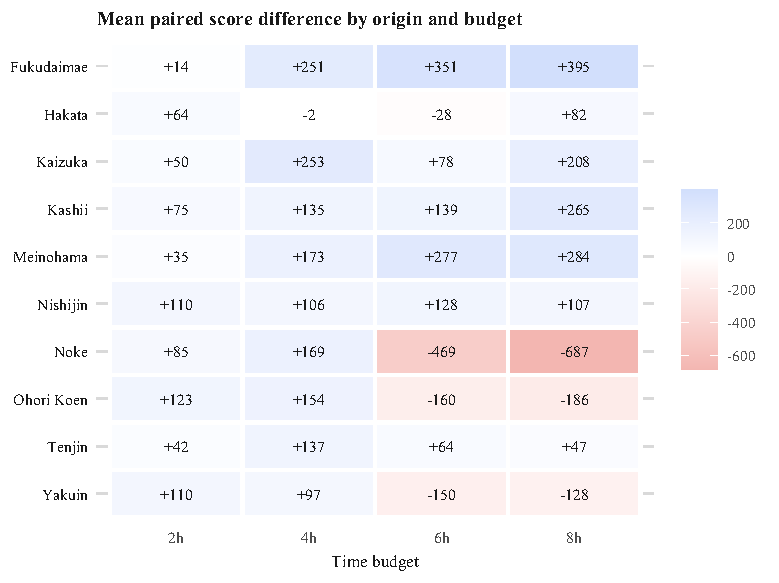
\includegraphics[width=\linewidth]{figures/exp1/underperformance_heatmap_20260723.pdf}
    \caption{Mean paired Stop Score gap (ReRAPTOR minus NSGA-II) by origin and
    budget. Each cell averages 15 matched tasks (three departures and five
    reward seeds); blue favors ReRAPTOR and red favors NSGA-II. Algorithm failures
    remain zero-score outcomes under the primary all-task policy.}
    \label{fig:exp1_underperformance}
\end{figure}

\begin{figure*}[t]
    \centering
    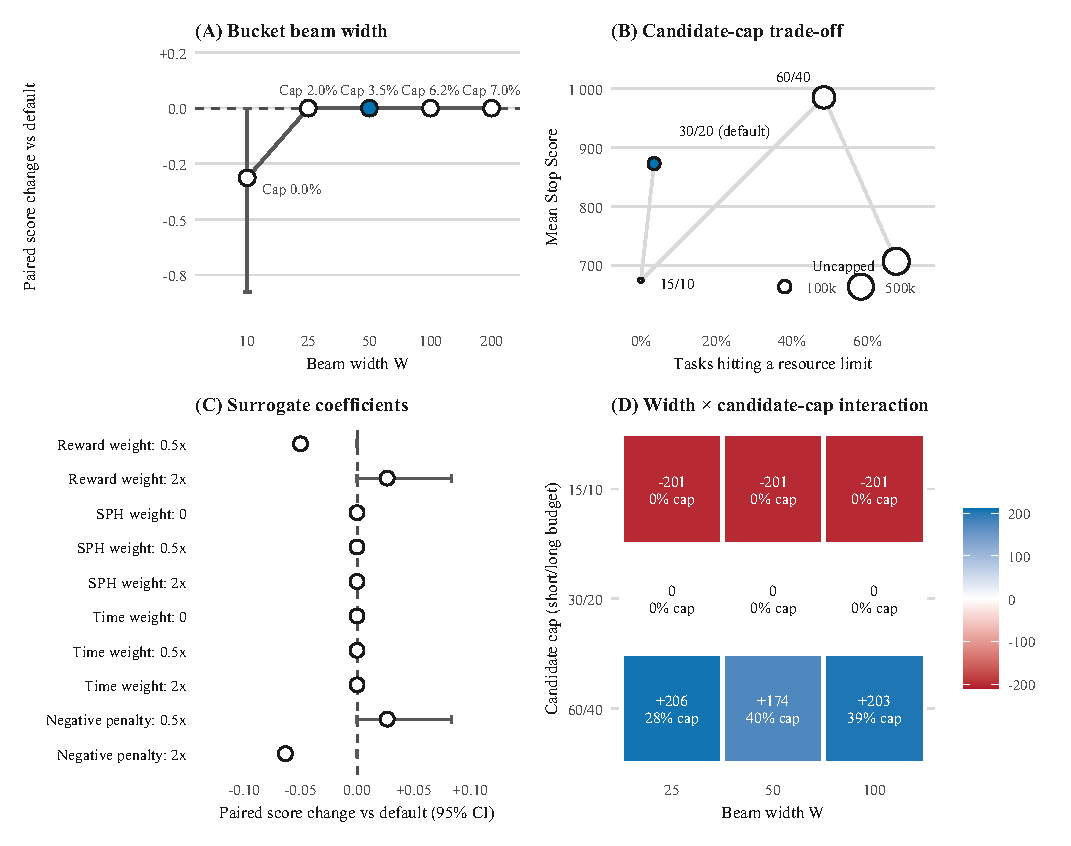
\includegraphics[width=0.92\textwidth]{figures/exp3/exp3_hyperparameter_sensitivity.pdf}
    \caption{Canonical hyperparameter sensitivity. (A) Paired score change and
    95\% crossed block-bootstrap interval across bucket beam widths; labels give
    resource-cap incidence. (B) Candidate-cap quality--resource trade-off, with
    point area proportional to generated labels. (C) Paired coefficient effects.
    (D) Confirmatory width--candidate-cap interaction; cells report mean score
    change from the \(W=50\), cap-\(30/20\) subset default and cap incidence.}
    \label{fig:exp3_sensitivity}
\end{figure*}

NSGA-II has \(288/3000\) algorithm-seed failures affecting 148 tasks. On the
452 tasks where all five runs succeed, the mean gap is \(+4.708\) (95\% CI
\([-63.024,67.875]\)); averaging its feasible seeds gives \(-3.059\) over 581
tasks (95\% CI \([-71.301,62.440]\); Supplementary Table~S1). Thus, the primary result includes
feasible-route reliability; successful-run solution quality is inconclusive.

\subsection{Experiment 2: Three-Component Search-Control Ablation and Supporting Evidence}
Experiment~2 disables the Beam layer, Dominance, and Negative down-ranking
individually and jointly from \texttt{Full}, which has all three controls
enabled, on the same 600 tasks (eight configurations; 4,800 runs).
\texttt{NoNeg}, \texttt{NoDom}, and \texttt{NoBeam} disable the named
components; hyphenated names disable all listed components. We report score,
generation time, generated labels, and \texttt{CapHit},
the fraction stopped by the 60-s timeout or 1,000,000-label no-pruning cap.

\begin{table}[t]
    \centering
    \caption{Canonical Experiment 2 ablation (means over 600 matched tasks).
    Generation is solver wall time; Labels counts the initial label plus every label
    created by edge extension before later Dominance/Beam removal; CapHit is the
    percentage stopped by the 60-s timeout or the triple-disabled configuration's
    1,000,000-label cap.}
    \label{tab:exp2_main_ablation}
    \resizebox{\linewidth}{!}{%
        \begin{tabular}{lrrrr}
            \toprule
            Method                    & Stop Score & Generation (ms) & Labels & CapHit (\%) \\
            \midrule
            Ours (Full)               & 872.438   & 10288.03     & 91,447    & 4.67        \\
            Ours (NoNeg)              & 872.472   & 11433.06     & 93,642    & 5.50        \\
            Ours (NoDom)              & 787.458   & 24141.25     & 219,676   & 16.00       \\
            Ours (NoBeam)             & 705.717   & 43041.76     & 539,463   & 67.67       \\
            Ours (NoBeam-NoDom)       & 299.873   & 56597.52     & 882,480   & 91.67       \\
            Ours (NoDom-NoNeg)        & 798.042   & 20688.47     & 231,871   & 11.67       \\
            Ours (NoBeam-NoNeg)       & 790.943   & 42042.27     & 1,000,717 & 65.50       \\
            Ours (NoBeam-NoDom-NoNeg) & 300.588   & 41234.67     & 903,851   & 91.17       \\
            \bottomrule
        \end{tabular}}
\end{table}

Table~\ref{tab:exp2_main_ablation} shows why the combination works. Removing
Dominance lowers score by \(84.98\), multiplies time by \(2.35\), and labels by
\(2.40\). Disabling the entire Beam layer (\texttt{NoBeam}), meaning candidate
trimming and bucket beam together, lowers score by \(166.72\), multiplies time
by \(4.18\) and labels by \(5.90\), and raises limit incidence from \(4.67\%\)
to \(67.67\%\). Without Beam and Dominance, \(91.67\%\) hit a limit and score
falls by \(572.57\), because productive deep search rarely finishes.
\texttt{NoBeam} is slightly better at 2h but \(8.71\times\) slower; every 6h
and 8h task times out (Supplementary Table~S4).

The Beam layer and Dominance are therefore complementary scalability controls.
Negative down-ranking is objective-specific: \texttt{NoNeg} ties Full on
594/600 tasks and improves six by only \(0.03\) points on average, so no generic
gain is established here (Supplementary Table~S4, Panel B).

\subsection{Experiment 3: Balance and Hyperparameter Sensitivity}
\paragraph{Balance and rationale.}
For a method with score \(s\) and generation wall time \(t\) on a base query, define
\(g_s=(s_{\max}-s)/(s_{\max}-s_{\min})\) and
\(g_t=(t-t_{\min})/(t_{\max}-t_{\min})\), where each extremum is taken across
methods for that query (a zero range gives zero loss). ReRAPTOR has the smallest
mean ideal distance \(d=\sqrt{g_s^2+g_t^2}\) (\(0.1315\), versus \(0.7413\) for
NSGA-II) and is both higher-scoring and faster in \(92/120\) queries. We test
whether \(W=50\), the candidate cap, or label-ranking coefficients drive the
result. The two ideal distances and the \(92/120\) count are reported in
Supplementary Table~S5.

The one-at-a-time (OAT) panel uses the same 600 tasks per configuration. It tests
beam widths of 10, 25, 50, 100, and 200; short/long-budget caps of 15/10,
30/20, and 60/40, or no cap; reward coefficients of 5,000, 10,000, and
20,000; SPH coefficients of 0, 2.5, 5, and 10; effective-time coefficients of
0, 0.05, 0.1, and 0.2; and Negative-penalty scales of 0.5, 1, and 2.
The inactive budget-overrun coefficient is not varied because hard feasibility
makes its term zero. The candidate-priority weights in
Eq.~\ref{eq:edge_priority} remain fixed and are outside this panel.

OAT differences use exact matched-task pairs and 20,000 crossed block-bootstrap
replications over reward seeds and origin--departure blocks. A confirmatory
\(3\times3\) panel crosses \(W\in\{25,50,100\}\) with caps \(15/10\),
\(30/20\), and \(60/40\) on a 72-task subset. Runs are sequential on the same
workstation; paired score and resources are primary. The OAT panel has 18
configurations (10,800 runs); the interaction panel reuses five OAT center cells
and adds four corners (288 runs), totaling 22 configurations and 11,088 verified runs.

\paragraph{Results and interpretation.}
Figure~\ref{fig:exp3_sensitivity} and Supplementary Table~S5
show width stability.
\(W=25,100,200\) reproduce the default score \(872.438\) on all 600 tasks;
\(W=10\) differs on eight and changes the mean by \(-0.313\) (95\% CI
\([-0.827,0]\)). Limit incidence rises from \(0.00\%\) at \(W=10\) to
\(2.00\%\), \(3.50\%\), \(6.17\%\), and \(7.00\%\) at
\(W=25,50,100,200\), respectively. Thus, 50 is a conservative middle default,
not a unique optimum; \(W=25\) is a lower-resource alternative. The taskwise
win/tie/loss counts are shown in Supplementary Table~S5, Panel B.

Candidate trimming controls the main trade-off. Tight caps \(15/10\) reduce
mean score to \(674.56\) (paired \(-197.88\), 95\% CI
\([-232.49,-164.07]\)) but eliminate limit hits. Caps \(60/40\) raise it to
\(984.87\) (\(+112.43\), 95\% CI \([+62.18,+171.16]\)) with 362,108 mean
labels and \(48.50\%\) limit incidence. With no cap, score falls to \(706.69\)
and \(67.67\%\) exhaust a limit. The default \(30/20\) lies between quality and
completion. In the interaction subset, widths remain equivalent at caps
\(15/10\) and \(30/20\); cap \(60/40\) adds \(174.04\)--\(206.33\) points but incurs
\(27.78\%\)--\(40.28\%\) limit incidence.

Surrogate coefficients have little effect. Halving or doubling the reward
weight changes the mean by \(-0.050\) or \(+0.027\); all SPH and time variants
reproduce the default; and penalty scales \(0.5\) and 2 change it by \(+0.027\)
and \(-0.063\). This matches the intended reward-first hierarchy. The
conclusion is robust over the tested widths and coefficients; the candidate cap
sets the material quality--resource boundary.

\subsection{Experiment 4: Route Case Study}
Three cases selected by fixed rules from the fixed 120-query results explain,
rather than extend, the statistics: Case~A is the largest lead where ReRAPTOR
is faster; B is its smallest score deficit when ranked first by ideal distance;
and C is its largest deficit among faster positive-score queries with a
ReRAPTOR/NSGA-II ratio of at least 0.8.

\begin{table*}[t]
    \centering
    \caption{Route cases. ``Stops'' counts unique scored non-origin stops;
    generation time uses the solver timing boundary defined in Section~5.1.}
    \label{tab:route_cases}
    \footnotesize
    \setlength{\tabcolsep}{4pt}
    \begin{tabular}{@{}llrrrrrrl@{}}
        \toprule
        Case & Query & \multicolumn{3}{c}{ReRAPTOR} &
        \multicolumn{3}{c}{Comparator} & Explanation \\
        \cmidrule(lr){3-5}\cmidrule(lr){6-8}
        & & Score & Gen. time & Stops & Method & Score & Gen. time & \\
        \midrule
        A & Fukudaimae, 07:00, 8h & 1455 & 13.83 s & 21 & NSGA-II & 684 & 31.75 s & broader coverage \\
        B & Kashii, 10:00, 2h & 375 & 115.79 ms & 6 & Pure RAPTOR & 376 & 10.92 s & near both ideals \\
        C & Ohori-koen, 14:00, 8h & 1479 & 4.11 s & 21 & NSGA-II & 1680 & 50.92 s & lower reward density \\
        \bottomrule
    \end{tabular}
\end{table*}

Table~\ref{tab:route_cases} links results to route behavior.
Case~A gains mainly by scoring 21 stops rather than 11. In Case~B,
ReRAPTOR keeps \(99.73\%\) of Pure RAPTOR's score while running
\(94.30\times\) faster. Greedy is faster still (0.85 ms) but scores only 263,
so ReRAPTOR provides the intermediate quality--time balance. In Case~C,
NSGA-II visits one fewer scored stop but
earns \(84.00\) points per stop versus \(70.43\); trimming can discard a partial
route that later reaches a valuable long-budget sequence. Supplementary
Table~S6 gives every numerical value used in these comparisons;
Supplementary Fig.~S1 gives the selection rules and route maps.

\section{Discussion}
\subsection{What the Experiments Establish}
The evidence supports a quality--resource claim, not universal route
superiority. Experiment~1 shows the aggregate gain and associates it with more
distinct scored stops and reliable feasible-route generation, not higher reward
per stop. Successful-run comparisons are inconclusive, and several long-budget
origins favor NSGA-II.

Experiment~2 supplies the mechanism: the Beam layer bounds
outgoing edges and retained labels, while Dominance removes locally weaker
labels. Without them,
resource limits interrupt deeper search, explaining why their combination can
raise completed-route score while reducing time. \texttt{NoNeg} is effectively
tied with Full, so the optional penalty has no generic benefit here.
Experiment~3 shows that this account is stable across tested widths and
label-ranking coefficients, while the candidate cap sets the
quality--completion boundary. The sensitivity claim is limited to the tested
panel: the edge-priority weights in Eq.~\ref{eq:edge_priority}, the 120-min
schedule lookahead, the depth rule, the transfer buffer, and the resource
thresholds remain fixed.

\subsection{Generalisability and Limitations}
The seeded rewards create a controlled search benchmark, not an estimate of
tourist satisfaction. An application can replace them with attraction ratings,
preferences, or event value without changing the timetable backbone. However,
independent stationary rewards omit spatial correlation, opening hours,
time-dependent value, heterogeneous users, crowding, diversity, and stop
interactions. The results concern reproducible value fields, not realized
visitor utility.

Two categories define scope. Method-level properties do not rely
on Fukuoka: labels retain reward-relevant history, candidate trimming and bucket
beam limit different stages, Dominance compares reward and time within a bucket,
and the reward module is replaceable. These are component functions, not
network-independent effect sizes; Dominance may still discard a history that
later becomes valuable. Empirical effect sizes, difficult origins and budgets,
limit rates, and useful width--cap settings may depend on Fukuoka. Other service
frequencies, transfer patterns, topologies, and observed utilities require tests
before any universal performance claim.

\section{Conclusion}
ReRAPTOR places a pluggable value model inside timetable-feasible expansion,
retains route history, and controls the richer search through the Beam layer
and heuristic
Dominance. On the Fukuoka benchmark, its mean Stop Score is \(872.438\),
\(8.710\%\) above NSGA-II, while NSGA-II requires \(6.89\times\) as much
generation time. Ablation identifies
the Beam layer and Dominance as the main scalability controls; sensitivity
identifies the
candidate cap as the main quality--resource parameter. Successful-run,
geographic, and route-case analyses bound the conclusion: ReRAPTOR offers a
strong overall balance here, but neither exact optimization nor universal
superiority.

\section*{Data and Code Availability}
The analysis code, canonical derived result files, figure inputs, and
reproduction instructions are publicly available at
\url{https://github.com/Akihito-zhou/reraptor_paper}.
The evaluated timetable snapshot is identified above by service date and file
name, and by a SHA-256 checksum in the repository's reproducibility record. The
snapshot was obtained through the Ekispert API and is not redistributed in the
public companion. Exact raw-input reproduction requires licensed provider
access and the authors' input-edge inventory. The released canonical outputs
and verifier support every displayed numerical claim without that proprietary
file.

\section*{Acknowledgment}
This study used transit schedule data for Fukuoka provided through the Ekispert
application programming interface (API;
\begin{CJK*}{UTF8}{min}Powered by Ekispert API\end{CJK*}).

\section*{Supplementary Materials}
Supplementary Tables~S1--S7 and Supplementary Fig.~S1 in the accompanying
\texttt{supplementary\_materials.pdf} provide numerical traceability for the
paired score interpretation, robustness and underperformance analyses,
budget-level ablation, sensitivity analysis, balance metrics, route cases, and
baseline configurations. Repository paths for every source are printed below
the corresponding supplementary table.

\begingroup
\renewcommand{\small}{\fontsize{8.2}{8.7}\selectfont}
\enlargethispage{6\baselineskip}
\bibliographystyle{spmpsci}
\bibliography{references_draft}
\endgroup

\end{document}
% end of file template.tex
